\documentclass{article}
\usepackage{amsmath, tikz, enumerate, sfmath, bm, multicol}
\renewcommand{\familydefault}{\sfdefault}
\usepackage[margin = 0.5in]{geometry}
\pagestyle{empty}
\raggedright
\tikzset{>=stealth}
\newcounter{Answers}
\begin{document}

\subsection*{Vectors and Matrices: Adding, Subtracting, and Scalar Multiplication P-Set}

Given $\vec{a} = \begin{bmatrix} -2 \\ 3 \end{bmatrix}$, $\vec{b} = \begin{bmatrix} 4 \\ 1 \end{bmatrix}$, $\vec{c} = \begin{bmatrix} 0 \\ -1 \end{bmatrix}$, and $\vec{d} = \begin{bmatrix} 2 \\ 1 \\ -3 \end{bmatrix}$, find each of the following (if possible).    \newline\\

\begin{tabular}{p{0.2\textwidth}p{0.2\textwidth}p{0.2\textwidth}}
1. \quad $\vec{a} + \vec{b}$    &
2. \quad $\vec{b} + \vec{c}$    &
3. \quad $\vec{c} - \vec{d}$      \\[10pt]
4. \quad $\vec{b} - \vec{a}$    &
5. \quad $2\vec{c}$             &
6. \quad $-3\vec{d}$            \\[10pt]
\end{tabular}


Write your answers for each using basis vectors $\hat{\imath}$ and $\hat{\jmath}$. Then draw your vector in the coordinate plane. \newline\\

\begin{tabular}{p{0.2\textwidth}p{0.2\textwidth}p{0.2\textwidth}}
7. \quad $\vec{a} + \vec{b}$    &
8. \quad $\vec{b} - \vec{a}$    &
9. \quad $2\vec{c}$             \\[15pt]
\end{tabular}

Given $A = \begin{bmatrix} 3 & -1 \\ 1 & -2 \end{bmatrix}$, $B = \begin{bmatrix} -4 & 0 \\ -3 & 2 \end{bmatrix}$, and $C = \begin{bmatrix} 1 & -2 & 3 \\ -1 & 2 & 2 \end{bmatrix}$, find each of the following (if possible).  \\[0.2in]

\begin{tabular}{p{0.2\textwidth}p{0.2\textwidth}p{0.2\textwidth}}
10. \quad $A + B$   &
11. \quad $B - C$   &
12. \quad $3C$      \\[10pt]
13. \quad $4A + 2B$ &
14. \quad $-2A$     &
15. \quad $B + 2A$  \\[15pt]
\end{tabular}

16. \quad Using matrix $C$ above, draw $C$ and $3C$ in the same coordinate plane.

\newpage

\textsc{Vectors and Matrices: Adding, Subtracting, and Scalar Multiplication P-Set}

\begin{multicols}{3}
\begin{enumerate}
 \setlength\itemsep{10pt}
     \item $\begin{bmatrix} 2 \\ 4 \end{bmatrix}$
     \item $\begin{bmatrix} 4 \\ 0 \end{bmatrix}$
     \item Not possible
\setcounter{Answers}{\value{enumi}}
\end{enumerate}
\end{multicols}
\vspace{0.2in}
\begin{multicols}{3}
\begin{enumerate}
\setcounter{enumi}{\value{Answers}}
     \item $\begin{bmatrix} 6 \\ -2 \end{bmatrix}$
     \item $\begin{bmatrix} 0 \\ -2 \end{bmatrix}$
     \item $\begin{bmatrix} -6 \\ -3 \\ 9 \end{bmatrix}$
\setcounter{Answers}{\value{enumi}}
\end{enumerate}
\end{multicols}
\vspace{0.2in}

\begin{multicols}{3}
\begin{enumerate}
\setcounter{enumi}{\value{Answers}}
     \item $2\hat{\imath} + 4\hat{\jmath}$   \newline\\
     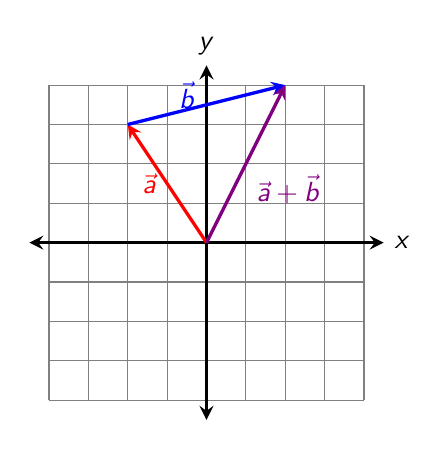
\begin{tikzpicture}[scale=0.5]
     \draw[gray] (-4,-4) grid (4,4);
     \draw[<->, very thick] (-4.5,0) -- (4.5,0) node [right] {$x$};
     \draw[<->, very thick] (0,-4.5) -- (0,4.5) node [above] {$y$};
     \draw[->, very thick, red] (0,0) -- node [midway, left] {$\vec{a}$} (-2,3);
     \draw[->, very thick, blue] (-2,3) -- (2,4);
     \node [blue] at (-0.5,3.75) {$\vec{b}$};
     \draw[->, very thick, violet] (0,0) -- node [midway, below right] {$\vec{a}+\vec{b}$} (2,4);
     \end{tikzpicture}
    
     \item $6\hat{\imath} - 2\hat{\jmath}$
     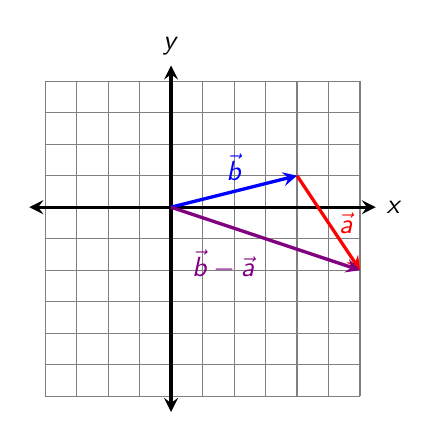
\begin{tikzpicture}[scale=0.4]
     \draw[gray] (-4,-6) grid (6,4);
     \draw[<->, very thick] (-4.5,0) -- (6.5,0) node [right] {$x$};
     \draw[<->, very thick] (0,-6.5) -- (0,4.5) node [above] {$y$};
     \draw[->, very thick, red] (4,1) -- node [midway, right] {$\vec{a}$} (6,-2);
     \draw[->, very thick, blue] (0,0) -- node [midway, above] {$\vec{b}$} (4,1);
     \draw[->, very thick, violet] (0,0) -- node [midway, below left] {$\vec{b}-\vec{a}$} (6,-2);
     \end{tikzpicture}
    
     \item $-2\hat{\jmath}$  \newline\\
     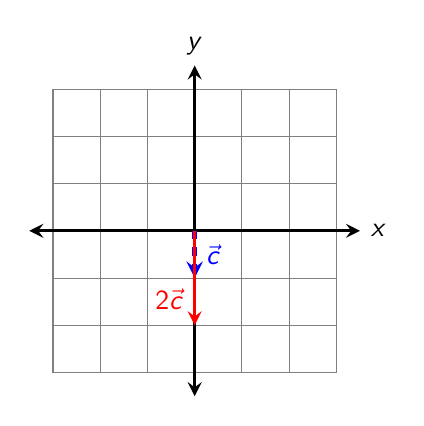
\begin{tikzpicture}[scale=0.6]
     \draw[gray] (-3,-3) grid (3,3);
     \draw[<->, very thick] (-3.5,0) -- (3.5,0) node [right] {$x$};
     \draw[<->, very thick] (0,-3.5) -- (0,3.5) node [above] {$y$};
     \draw[->, ultra thick, dashed, blue] (0,0) -- node [midway, right] {$\vec{c}$} (0,-1);
     \draw[->, very thick, red] (0,0) -- node [midway, below left] {$2\vec{c}$} (0,-2);
     \end{tikzpicture}
\setcounter{Answers}{\value{enumi}}
\end{enumerate}
\end{multicols}
\vspace{0.2in}

\begin{multicols}{3}
\begin{enumerate}
\setcounter{enumi}{\value{Answers}}
     \item $\begin{bmatrix} -1 & -1 \\ -2 & 0 \end{bmatrix}$
     \item Not possible
     \item $\begin{bmatrix} 3 & -6 & 9 \\ -3 & 6 & -9 \end{bmatrix}$
\setcounter{Answers}{\value{enumi}}
\end{enumerate}
\end{multicols}
\vspace{0.2in}

\begin{multicols}{3}
\begin{enumerate}
\setcounter{enumi}{\value{Answers}}
     \item $\begin{bmatrix} 4 & -4 \\ -2 & -4 \end{bmatrix}$
     \item $\begin{bmatrix} -6 & 2 \\ -2 & 4 \end{bmatrix}$
     \item $\begin{bmatrix} 2 & -2 \\ -1 & -2 \end{bmatrix}$
\setcounter{Answers}{\value{enumi}}
\end{enumerate}
\end{multicols}
\vspace{0.2in}

\begin{enumerate}
\setcounter{enumi}{\value{Answers}}    
    \item \quad \newline\\
    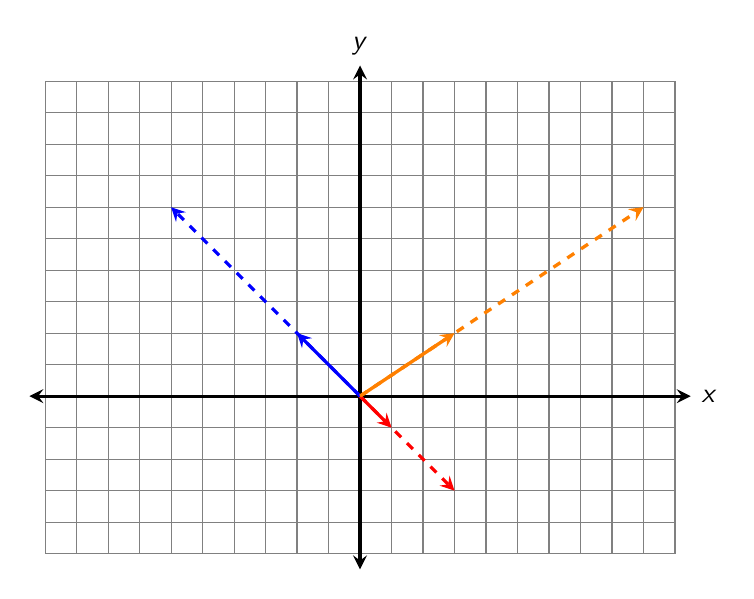
\begin{tikzpicture}[scale=0.4]
    \draw[gray] (-10,-5) grid (10,10);
    \draw[<->, very thick] (-10.5,0) -- (10.5,0) node [right] {$x$};
    \draw[<->, very thick] (0,-5.5) -- (0,10.5) node [above] {$y$};
    \draw[->, very thick, red] (0,0) -- (1,-1);
    \draw[->, very thick, blue] (0,0) -- (-2,2);
    \draw[->, very thick, orange] (0,0) -- (3,2);
    \draw[->, dashed, very thick, red] (0,0) -- (3,-3);
    \draw[->, dashed, very thick, blue] (0,0) -- (-6,6);
    \draw[->, dashed, very thick, orange] (0,0) -- (9,6);
    \end{tikzpicture}
\end{enumerate}

\end{document}
